\subsubsection{Raspicontroller}
Auf dem Raspberry Pi läuft eine eigens geschriebene Software, welche sich Raspicontroller nennt. Einen Überblick über die angeschlossene Peripherie ist dem Blockdiagramm in Abbildung \ref{fig:blockdiagramm} zu entnehmen. Der Raspicontroller ist für den gesamten Vorgang des Ballwurfs zuständig. Die Applikation ist in Python geschrieben und wird als Service auf einem Raspberry Pi ausgeführt. Auf dem Raspberry Pi ist das Betriebssystem Arch Linux installiert. Arch Linux lässt sich ohne grafische Oberfläche betreiben, wodurch wenig Ressourcen verwendet werden. Das Betriebssystem lässt sich komplett über Textdateien konfigurieren. Der Raspberry Pi stellt einen Access Point zu Verfügung, damit man sich mit dem Fotoshoot UI drahtlos verbinden kann. Diese Schnittstellen werden über einen Webserver bereitgestellt. Die Steuerbefehle werden über eine REST-Schnittstelle entgegen genommen, welche detaillierte in Abschnitt \ref{sec:rest-schnittstelle} beschrieben sind. 
\\
\\
\textbf{Komponente Webserver}
Der Webserver wurde mit Hilfe der Python-Bibliothek \texttt{web.py} erstellt. Diese Komponente nimmt Anfragen entgegen und verarbeitet diese. In einer solchen Anfrage sind unterschiedliche Komponenten involviert. Beispiel: Abfrage der Log-Einträge. Der Webserver empfängt die Anfrage und leitet diese an die Logger-Komponente weiter.
\\
\\
\textbf{Komponente Detection}
Um den Korb zu erkennen wird ein Foto geschossen und ein Algorithmus erkennt die Position des Korbes. Der Algorithmus wurde selbst entwickelt und in Python implementiert. Abbildung \ref{fig:ablauf-ortung-des-korbes-algorithmus} zeigt den grundsätzlichen Ablauf des Algorithmus.

\begin{figure}[h!]
	\centering
	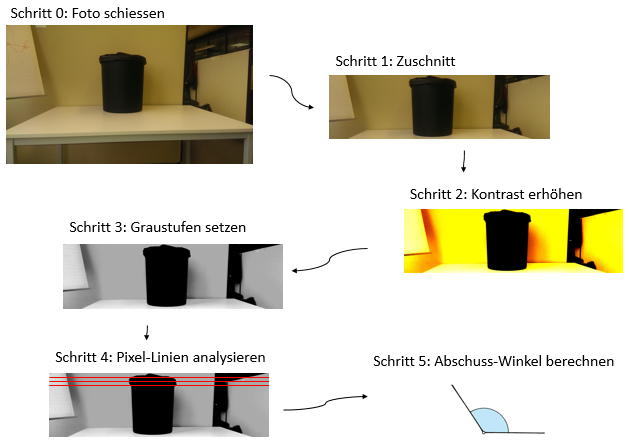
\includegraphics[width=0.7\linewidth]{../../fig/ablauf-ortung-des-korbes-algorithmus}
	\caption{Ablauf Erkennung des Korbes}
	\label{fig:ablauf-ortung-des-korbes-algorithmus}
\end{figure}

\newpage
Sobald klar ist wo der Korb im Bild steht, werden die Pixel-Koordinaten zu Anzahl Schritte für den Schrittmotor umgerechnet. In der Tabelle \ref{tab:berechnung-steps} ist die Berechnung ersichtlich. 

\begin{table}[h!]
	\renewcommand{\arraystretch}{1.5}
	\centering
	\begin{tabular}{l l}
		Anzahl Stepper Schritte für 360$^\circ$ & 200 Schritte \\
		Stepper $\frac{Winkel}{Schritt}$ & $\frac{360}{200} = 1.8^\circ$ \\
		Übertragung & $\frac{22}{290} = 0.0759$ \\
		Effektives $\frac{Winkel}{Schritt}$ & $w = 1.8 \cdot 0.0759 = 0.1365^\circ = 0.0023736 Rad$ \\
		HalbeBildPixelBreite & $c = \frac{width}{2}$ \\
		HalbeBildCmBreite & $d = 99*(1-\frac{Zuschnitt}{640})$ \\
		Position der Korb in Pixel & $x$ \\
		Pixel Abstand von der Mitte & $x - c$ \\
		Abstand in Cm Korb-Bildmitte & $k = \frac{d}{c} \cdot (x-c)$ \\
		Abstand Maschine-Wand & $a = 190$ cm \\
		Winkel & $\alpha = arctan\frac{k}{a}$ rad \\
		Anzahl Schritte & $\frac{\alpha}{w}$ \\
	\end{tabular}
	\label{tab:berechnung-steps}
	\caption{Berechnung Anzahl Schritte für den Schrittmotor}
\end{table}

\noindent
\textbf{Komponente Camera}
Mit dem Raspberry Pi wird eine Kamera über die CSI-Schnittstelle\footnote{Camera Serial Interface} verbunden. Die Kamera wird mit der Python-Bibliothek \texttt{picamera} angesteuert. Diese Bibliothek liefert das Bild als Python-Objekt zurück, welches danach direkt dem Algorithmus übergeben werden kann.
\\
\\
\textbf{Komponente Serial}
Hier ist eine Abstraktionsebene für den Webserver implementiert. Diese gilt als Vermittler zwischen Freedom-Board und Webserver. Das Freedom-Board wird über eine serielle Schnittstelle mit der Python-Bibliothek \texttt{pyserial} angesteuert.
\\
\\
\textbf{Komponente Freedom}
Das Freedom-Board, welches zuständig für die Motoren ist, ist über USB angeschlossen. Im Elektrotechnik-Bereich wird explizit auf das Freedom-Board eingegangen. Die Schnittelle ist in Abschnitt \ref{sec:schnittstelle-raspi-freedom} dokumentiert.
\\
\\
\textbf{Komponente Logger}
Diese Komponente ist zuständig für das Logging der Applikation. Log-Einträge werden entgegengenommen und in eine Datei gespeichert. Diese Einträge können entsprechend auch gelesen werden.
